\section{Zadanie 2}

\subsection{Charakterystyka algorytmu Neville'a}

Algorytm Neville'a to metoda numeryczna służąca do wyznaczania wartości interpolowanego wielomianu w danym punkcie. Główną zaletą tej techniki jest możliwość efektywnego obliczania wartości wielomianów na podstawie zadanego zestawu punktów, choć jej złożoność obliczeniowa wynosi \( O(n^2) \), co może być kosztowne przy dużych zbiorach danych.

Interpolacja w algorytmie Neville'a bazuje na rekurencyjnym wzorze, który pozwala obliczyć wartość funkcji w punkcie \( x \) na podstawie danych punktów \( (x_i, y_i) \). Testy przeprowadzono, losując \( n \) punktów z ustalonego przedziału \( D = (0, 10) \), a następnie porównując wartości interpolacji z rzeczywistymi wartościami funkcji w 100 równomiernie rozłożonych punktach.

Eksperyment wykonano dla czterech funkcji:
\begin{itemize}
    \item Funkcja trygonometryczna: \( f(x) = \sin(x) + \cos(x) \),
    \item Wielomian 3 stopnia: \( f(x) = x^3 - 2x + 1 \),
    \item Funkcja wykładnicza: \( f(x) = e^x \),
    \item Funkcja wymierna: \( f(x) = \frac{1}{1 + x^2} \).
\end{itemize}

Dla każdej funkcji obliczono błąd interpolacji oraz odchylenie standardowe, a także czas wywołania algorytmu.

\subsection{Wyniki i wnioski}

% trygonometryczne
\begin{center}
\textbf{Wyniki dla funkcji trygonometrycznej:}  
Najmnieszy błąd: \( 2.01 \times 10^{-13} \pm 1.03 \times 10^{-12} \)  przy 23 punktach  

\begin{minipage}{0.49\textwidth}
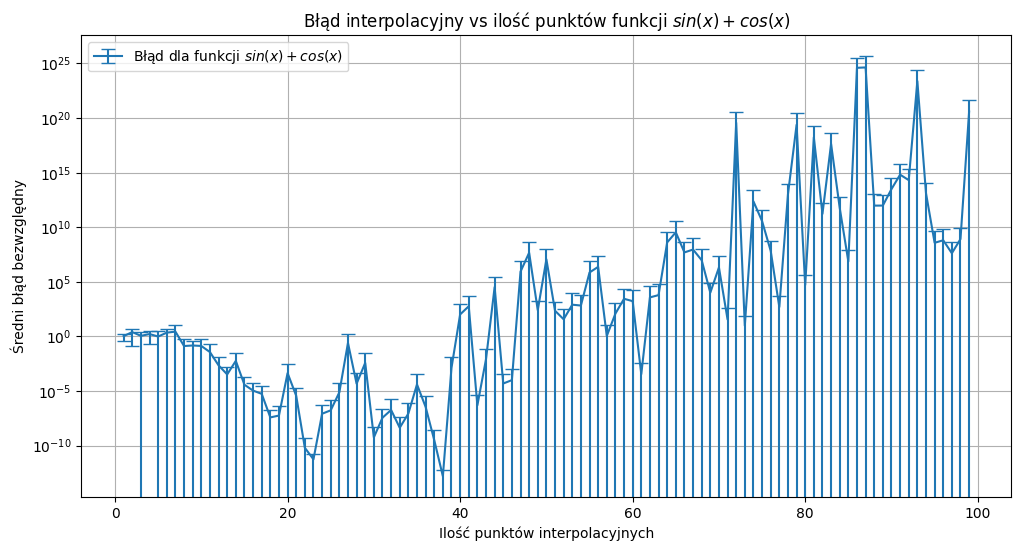
\includegraphics[width=\textwidth]{wykresy/zadanie 2/blad_tryg.png}
\end{minipage}
\begin{minipage}{0.49\textwidth}
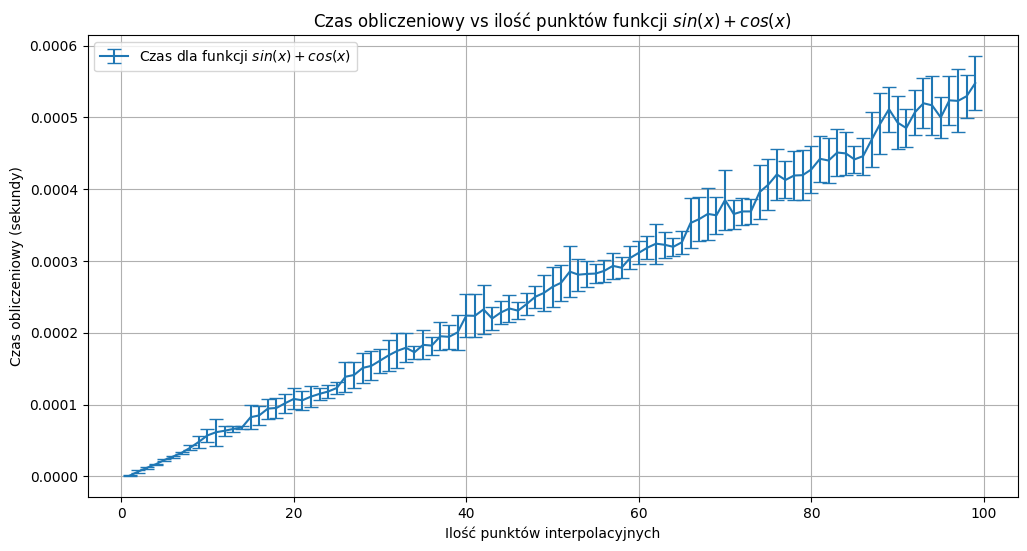
\includegraphics[width=\textwidth]{wykresy/zadanie 2/czas_tryg.png}
\end{minipage}

% wielomian 3 rzędu
\textbf{Wyniki dla wielomianu trzeciego rzędu:}  
Najmniejszy błąd: \( 8.21 \times 10^{-14} \pm 1.31 \times 10^{-13} \)  
przy 9 punktach.  

\begin{minipage}{0.49\textwidth}
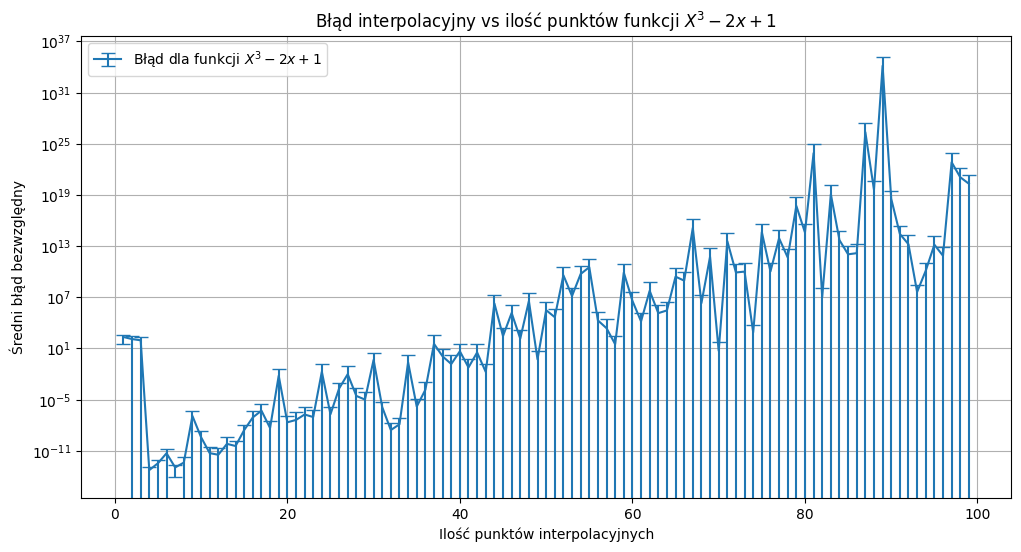
\includegraphics[width=\textwidth]{wykresy/zadanie 2/blad_wiel.png}
\end{minipage}
\begin{minipage}{0.49\textwidth}
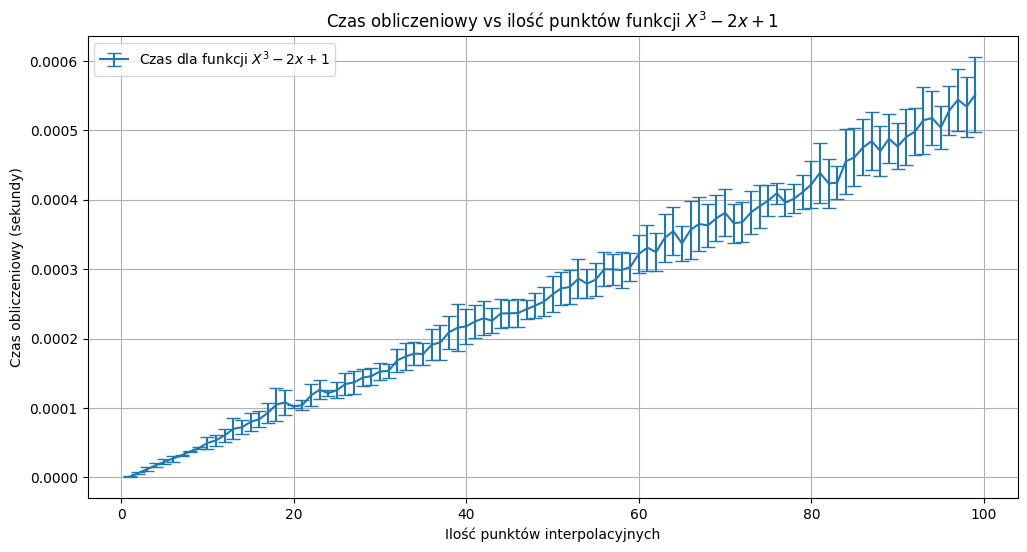
\includegraphics[width=\textwidth]{wykresy/zadanie 2/czas_wiel.png}
\end{minipage}

% exponenta
\textbf{Wyniki dla funkcji exp:}  
Najmniejszy błąd: \( 2.00 \times 10^{-9} \pm 1.25 \times 10^{-8} \)  
przy 26 punktach. 

\begin{minipage}{0.49\textwidth}
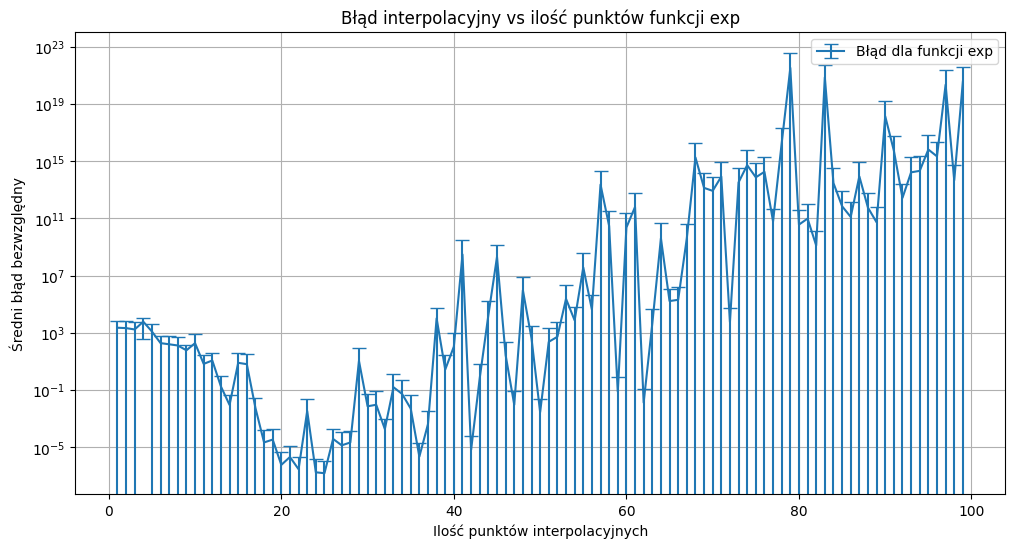
\includegraphics[width=\textwidth]{wykresy/zadanie 2/blad_exp.png}
\end{minipage}
\begin{minipage}{0.49\textwidth}
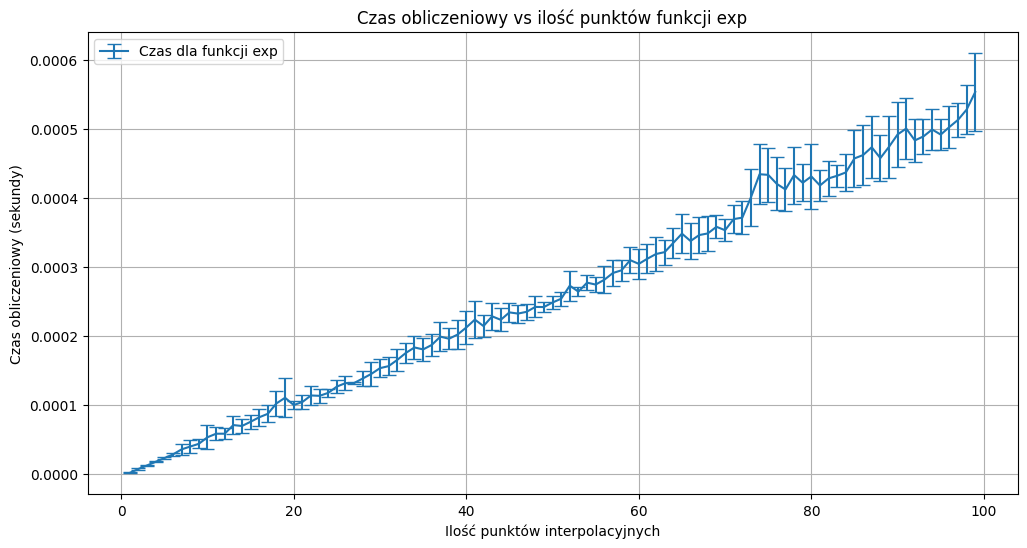
\includegraphics[width=\textwidth]{wykresy/zadanie 2/czas_exp.png}
\end{minipage}

% funkcja wymierna
\textbf{Wyniki dla funcji $\frac{1}{1 + x^2}$:}  
Najmniejszy błąd: \( 7.63 \times 10^{-12} \pm 3.28 \times 10^{-11} \)  
przy 28 punktach.

\begin{minipage}{0.49\textwidth}
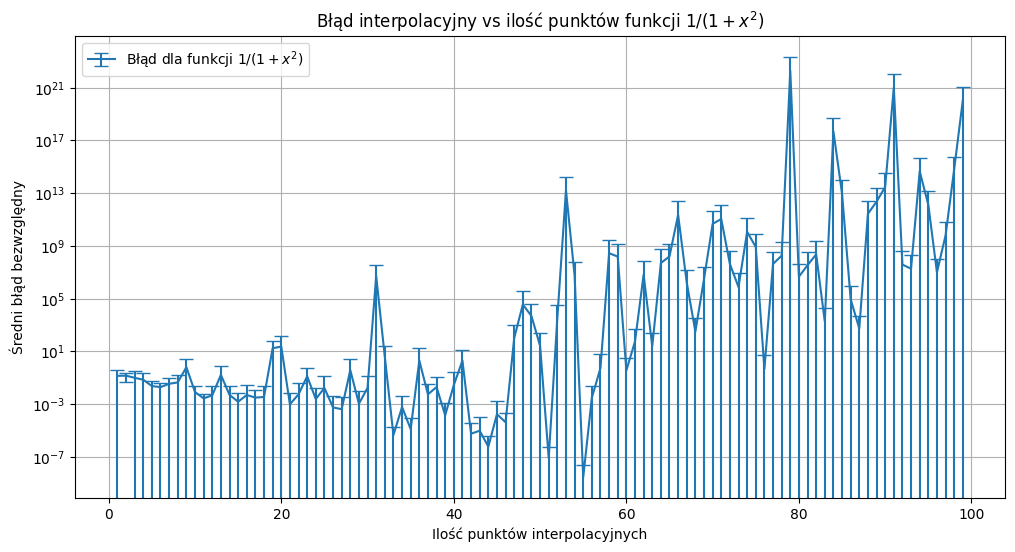
\includegraphics[width=\textwidth]{wykresy/zadanie 2/blad_wym.png}
\end{minipage}
\begin{minipage}{0.49\textwidth}
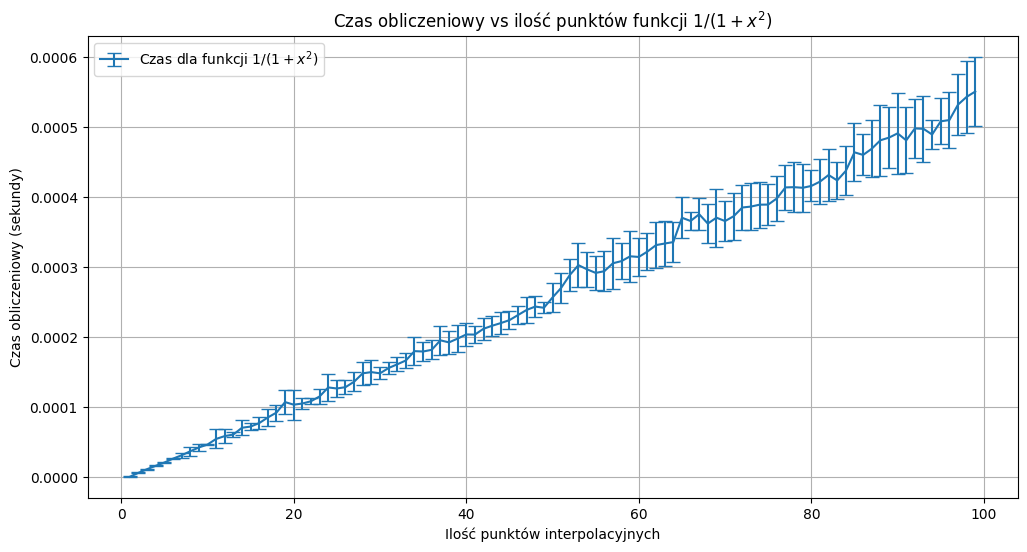
\includegraphics[width=\textwidth]{wykresy/zadanie 2/czas_wym.png}
\end{minipage}
\end{center}

\textbf{Wnioski:}
\begin{itemize}
    \item \textbf{Precyzja dla 10–20 punktów:} Przy wyborze od 10 do 20 punktów osiągano najlepsze wyniki pod względem dokładności, ponieważ przy większej liczbie punktów wzrastają błędy, głównie z powodu efektów numerycznych wynikających z dużych wartości przyrostów. Widzimy jednak duże odchylenie standardowe 
    \item \textbf{Czas obliczeń:} Czas wykonania algorytmu Neville'a był liniowy w zależności od liczby punktów, z bardzo małym współczynnikiem przyrostu. Wynika to z implementacji.
    \item \textbf{Różnice między funkcjami:} Największe błędy zaobserwowano w przypadku funkcji wykładniczej, co wynika z jej szybkiego wzrostu w przedziale \( D \). Najmniejsze błędy odnotowano dla wielomianu sześciennego, co jest zgodne z oczekiwaniami, gdyż metoda interpolacji wielomianowej jest idealna dla funkcji tego typu.
    \item \textbf{Odchylenie standardowe, błąd} Dziwne pokazywanie odchylenia standardowe jest spowodowane, przeskalowaniem wykresu. Głównie niesie informacje czy wyskakuje ono znacznie w górę. 
\end{itemize}
